\subsection{Elasticsearch Architecture}
To achieve scalability across multiple machines,
the second implementation of query expansion was done using Elasticsearch.
The initial thought was to implement query expansion directly into Elasticsearch's core.
However, during the research phase it was discovered that Elasticsearch has a plugin API.

The query expansion plugin for Elasticsearch is almost identical to the implementation described in subsection \ref{sec:algorithm} and in subsection \ref{sec:lucene}.
Thus, this subsection will only describe the differences.
The differences is mostly how the documents are indexed and how the queries are structured.

Figure \ref{fig:sequence-diagram-elasticsearch} displays the sequence diagram for the implemented Elasticsearch plugin.
First the query arrives the coordination node in the Elasticsearch cluster.
The query is parsed and distributed to all the relevant shards.
Each uses the plugin to calculate their local top-k documents.
Metadata of each shard is returned to the coordination node,
which again merges the results and calculates the global top-k documents.
Lastly,
the actual documents are retrieved from all the shards and the final result are returned.

\begin{figure}[h!]
  \centering 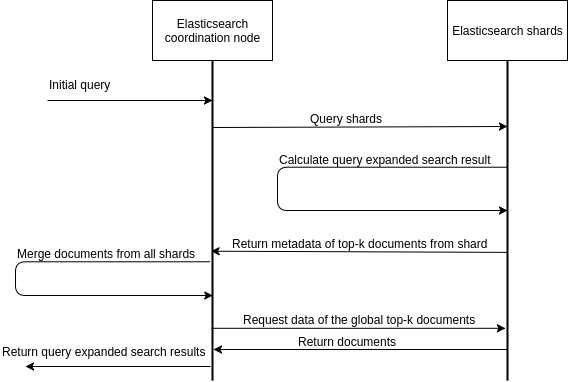
\includegraphics[width=1\linewidth]{img/sequence-diagram-elasticsearch.png}
  \caption{Sequence diagram for the Elasticsearch implementation.}
  \label{fig:sequence-diagram-elasticsearch}
\end{figure}

\subsubsection{Elasticsearch Plugin API}
Elasticsearch has it's own plugin API\footnote{\url{https://www.elastic.co/guide/en/elasticsearch/plugins/5.2/index.html}}.
This plugin API can be used to extend Elasticsearch's index and query capabilities.
The implementation described in this master thesis creates a plugin which extends the REST API with query expansion.
When a plugin is installed, the installation are done on all the nodes.
The plugin API has two main catogories: core plugins and community contributed plugins.
Core plugins are plugins which are a part of the Elasticsearch project.
These plugins are develop by the Elastic team.
Community contributed plugins, are plugins outside the Elasticsearch project.
These plugins are developed by the community.
When a plugin is installed,
the installation are distributed to all the nodes.
As the installation is distributed,
all the nodes are able to act as a coordination node,
which also makes the plugin API scalable.

Accessing the extended REST API is done sending a POST request to the URL \url{http://localhost:9200/_expansion}.
This URL assumes that the server is running locally and that Elasticsearch's default port 9200 is used.
\texttt{/\_expansion} is the new REST API extension.
To send a query, the POST request need to have a body as shown in listing \ref{lst:rest-api-extension}.
The body consists of a json object with one key value pair.
The key is \texttt{search\_query} and the key is the desired query string.
Query strings with containing multiple terms are divided into separate terms.
The terms are extracted by spliting the query string on the character "space".

\begin{lstlisting}[language=json, caption={The POST request body for the implemented query expansion.}, label={lst:rest-api-extension}]
{
  "search_query": "search terms"
}
\end{lstlisting}

\subsubsection{Elasticsearch Notes}
- The implementation decribed in this report belongs to the community contributed plugins.

- The implemented plugin extends the current Elasticsearch REST API.

- Architecture with Elasticsearch.

- Elasticsearch plugin to extend the Elasticsearch API.

- Elasticsearch plugin functionality

- Elasticsearch queries in java which are used

- Describe REST listener

- Describe the configration required to create an Elasticsearch plugin

\subsubsection{Indexing}
Many storage solutions requires the stored data types to be defined before inserting data.
Elasticsearch have support to both predefined data types and data types determined at index time.
Data types determined while indexing is called dynamic mapping, and predefined data types are called static mapping.
Dynamic mapping are useful when prototyping and developing.
However, dynamic mapping may assign wrong types to a field.
For instance one might have a geo location point.
A geo location point will most likely be sent to Elasticsearch as two floats, latitude and longitude.
It is fine to store the values as floats, but Elasticsearch have separate data type for latitude and longitude called Geo-point.

With static mapping on the other hand, every mapping type are defined before indexing.
Static mapping ensures that each field is assigned the correct mapping.
The mapping used in this master thesis is available in appendix \ref{ap:elasticsearch-mapping}.

\subsubsection{Searching}
All the searches in the Elasticsearch implementation is similar to the searches described in the Lucene implementation,
but there are a few important differences.
The query expansion algorithm requires three different types of search:
single term query, multiple term query and field stats query.

The first step of the algorithm is to retrieve the top-k documents.
In elasticsearch this is done as a multiple term query,
and the implemented Java code is available in appendix \ref{ap:multiple-term-query}.

Retrieving the number of times a term appears in the collection may be done through Elasticsearch's count API.
However, this API is not available through the Java client library.
Instead this information may be fetched using a normal single term query.
Metadata from the search result contains the needed information.
Listing \ref{ap:elasticsearch-metadata} displays an example on how the returned result may look.
The array \texttt{hits} is intentionally left out to keep the example short,
as the array contains the search result itself.
The search result consists of information about how long the search took, how many shards searched, the total number of hits,
the maximum returned document score and the search result itself.
In listing \ref{ap:elasticsearch-metadata} there is a field called \texttt{total},
which indicates the total number of hits the term query produced.

Lastly, the query expansion also requires to know the total number of terms in the collection.
This information can be retrieved using Elasticsearch's field stats API.
The API exposes native Lucene index function,
for retrieving metadata from the inverted index.

\begin{lstlisting}[language={json}, caption={Example of the metadata returned by Elasticsearch.}, label={ap:elasticsearch-metadata}]
{
  "took": 3,
  "timed_out": false,
  "_shards": {
    "total": 5,
    "successful": 5,
    "failed": 0
  },
  "hits": {
    "total": 2912,
    "max_score": 9.73782,
    "hits": [
      ...
    ]
  }
}
\end{lstlisting}
